\documentclass[border=2pt]{standalone}
\usepackage{pgfplots}
\pgfplotsset{compat=1.18}
\definecolor{red}{rgb}{0.7,0.11,0.11}
\definecolor{blue}{rgb}{0.0,0.20,0.42}
\definecolor{green}{rgb}{0.11,0.35,0.02}
\begin{document}
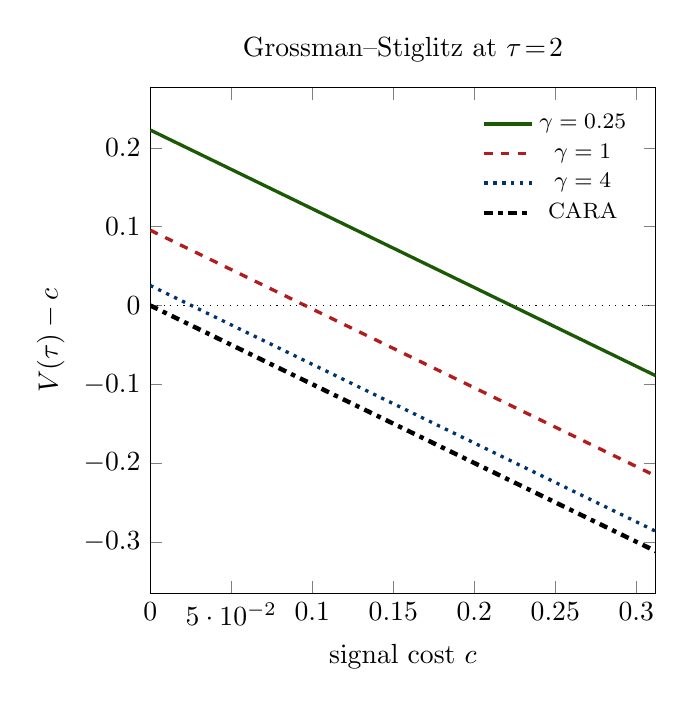
\begin{tikzpicture}
\begin{axis}[
    width=8cm, height=8cm,
    xmin=0, xmax=0.3119,
    xlabel={signal cost $c$},
    ylabel={$V(\tau)-c$},
    title={Grossman--Stiglitz at $\tau\!=\!2$},
    legend pos=north east,
    legend style={fill=none, draw=none, font=\footnotesize},
]
\addplot[very thick, color=green] coordinates {(0,0.222791)(0.3119,-0.089116)};
\addplot[very thick, color=red, dashed] coordinates {(0,0.095537)(0.3119,-0.216371)};
\addplot[very thick, color=blue, dotted] coordinates {(0,0.025348)(0.3119,-0.286560)};
\addplot[ultra thick, color=black, dashdotted] coordinates {(0,0)(0.3119,-0.3119)};
\addplot[thin, color=black, dotted]
    coordinates {(0,0)(0.3119,0)};
\addlegendentry{$\gamma = 0.25$}
\addlegendentry{$\gamma = 1$}
\addlegendentry{$\gamma = 4$}
\addlegendentry{CARA}
\end{axis}
\end{tikzpicture}
\end{document}
